%!TEX root = main.tex

\section{Starcraft}

\begin{figure}[h!tb]
\centering
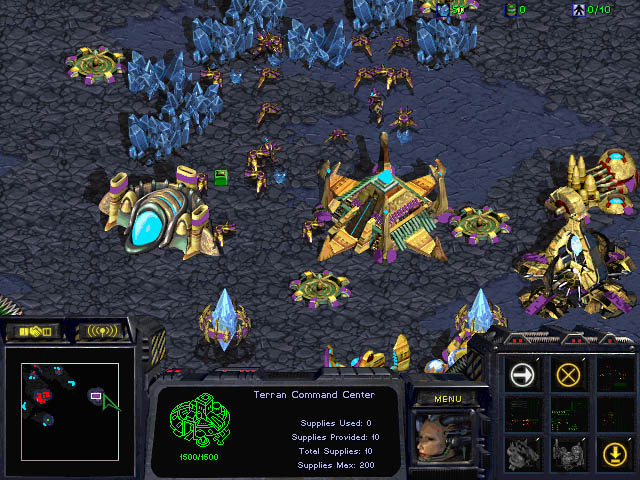
\includegraphics[scale=0.5]{graphics/scbw.jpg}
\caption{Star Craft Brood War}
\label{fig:scbwIntro}
\end{figure}

StarCraft is on the surface a very simple game, it has only three different playable races, a
handful of different buildings and units, and relatively simple to comprehend
goals. But once you start analyzing the game, the reality is quite different. The brood war expansion pack was released back in 1998, and has been played at a high level since that and all the way up to today. And the meta game has evolved during the entire lifespan of the game and is still changing today with new tactics showing up from tournament to tournament.
\cite{blizzardstarcraft}

When playing at a really high level you are working with really small windows of opportunity, often called timings. And it is these timings that enable a game with what should in theory be simple elements to have such complex and evolving strategies.

TODO: talk about supply and how it is different from race to race. 

\subsection{Terran}

\begin{quote}
Strengths: \\
Mobility, great defense, build anywhere, cloaking, versatility, Marines, strong through whole tech-tree, easy to learn, instant cloak detection, ability to repair buildings and most units. \\
Weaknesses: \\
Tendency to "turtle", need lots of space, require active scouting, require micromanagement for special abilities, vulnerable to Dark Swarm, buildings burn up when highly damaged. 


\cite{terranoverview}
\end{quote}

Terran are the human faction of StarCraft, a futuristic version of man today. They are known for high adaptability with a good variety of defensive and mobile armies. They are best known for their mobile biological armies, or their slow moving turtling tech(tanks) armies that slowly creeps across the map and secures section for section. This versatility makes them a great class with a lot of different possible strategies and combinations that can be effective. 

The Terran worker is the Space Construction Vehicle (SCV). This unit can gather minerals, build buildings and unique for the Terran race repair other mechanical units or buildings. When constructing buildings the unit has to work on the building from the initial placement to the building is complete, meaning it will be unable to perform other action in this time, and can be attacked. If the SCV halts construction or is killed, the building will have to be canceled or finished by another SVC. Like mentioned before it can also repair mechanical units like tanks if they have taken damage, but to perform this action they have to be pulled from other tasks like mining minerals so it is a two edged sword. Terran buildings will slowly self destruct if left at low health, so it is important to repair them if they have taken significant damage. 

Terran buildings also have a unique feature in that they can lift of the ground and fly around after being constructed. They can then land in a new location and continue production of units or upgrades. Some buildings can also create add-ons that unlocks new units and upgrades for that building. Terran also have a unique building in the bunker. This a a defensive building where  biological units can seek refuge while still attacking, but from a fortified position that protects them from damage. The bunker has to be taken out before the units inside can be damaged and killed. While being useless on it's own, the building can be a death trap when filled with infantry. The bunker can also be repaired by an SCV, like any other Terran building, so the SCVs have to be a priority for an attacking army before they can destroy the bunker. 

The health regeneration mechanics for the Terran race are twofold. The medic is used to heal biological units after they have suffered damage in battle, they can also heal other medics, but not them self. And mechanical units can be repaired by pulling SCVs from mining and using them to repair the unit. SCVs can also be effective to use in combat as they can repair the unit while it is taking damage, and several SCVs can repair the same unit at the same time for an increased regeneration rate. 

\subsection{Protoss}
The protoss are an technological advanced alien race that rely on psionic abilities and cybernetics in battle. Because they are the most technological advanced race in StarCraft they are known for their raw power. With powerful but expensive units they can crush their opponents on the battlefield with an outnumbered but superior quality army.

The protoss worker is called a probe, and is like the SCV used to gather minerals and build buildings. Protoss buildings are also not constructed, they are warped in from their home planet, so a probe only needs to place a warp beacon where the building should be placed and then it can return to mining minerals while the building warps in by it self. This allows the use of one probe for construction of several buildings at basically the same time, and then it can return right to mining. This can allow an protoss player to setup remote expansions in a short time with a single probe. 

In contrast to the terran race the protoss can't just build buildings anywhere, they have to place them on a power grid generated by a pylon, the protoss supply building. Pylons also power buildings so if an enemy takes out all the pylons around some production building it can no longer produce any units or research upgrades. The player will then have to build new pylons to power up the building again before he can continue production. 

Special for protoss units and buildings are that they have energy shields that protect them against damage and recharges to full strength over time. In order for an enemy to damage a protoss unit, it has to first deplete the shield that protects it only then can they proceed to damaging the unit itself. For an enemy it is then important to finish of the unit when it's shield is fully depleted or it will regenerate to full strength. 

\subsection{Zerg}
 The zerg are a race of very different creatures that have been united under a central intelligence called the Overmind. In their goal for power, they have been selectively evolved towards being very effective killers. Technologically they are far behind the other races, but they make up for this with a big army size and superior biological properties. 

 The zerg worker unit is called a drone. When construction a building a drone will sacrifice it self and mutates into the building. This means that for every building that the player constructs he looses a worker. In every other way they behave just the same as any other worker. For every race the worker unit is produced from the foundation building, for zerg this is the hatchery. But for zerg every other unit is also created from the hatchery, and any unit buildings that are constructed only unlocks the possibility to create that unit from the hatchery. This is because zerg have a mechanic called larva. They are produced by the hatchery over time, up to a maximum of three at a given time, and they can be morphed into another zerg unit that is unlocked. 

 Similar to protoss the zerg can't just build buildings anywhere, because the buildings are biological they require nourishment to function and has to be build on creep. Creep is produced by the Hatchery and Creep Colonies and then radiates outwards from these onto any fertile ground in the area. The Hatchery is the only building that can be built without creep, as it produces its own nourishment. 

 Zerg units and buildings have a unique ability to regenerate lost health over time if left alone. This means an attacker should finish of an attacked unit or it will come back with full health after a while. This also makes a tactical retreat important for the zerg players, as they can then rest their army to allow them to regenerate back to full health after taking damage in a battle. Burrowing is also a unique ability for the zerg units, and has great synergy with the health regeneration ability. This allows them to burrow in the ground to get out of harms way, and here they can regenerate health without worrying about taking damage. This also allows for ambush tactics by burrowing armies and waiting for the enemy before launching a surprise attack. It can even be used to gain map control by burrowing units in strategic places to scout that area. Only using some form of detector can the enemy see and attack units that have burrowed. 